\subsection{Signup}
\label{ssec:konzept:client:signup}
Um eine Umfrage erstellen zu können, an der Umfrageteilnehmer partizipieren können, muss zuvor ein Nutzerkonto erstellt werden. 
Hierfür wählt der Benutzer wie in Abb. \ref{fig:MockSignup} dargestellt das Formfeld mit seinem Benutzernamen wie z.B. \emph{\texttt{Martin}}. 
Danach wird die E-Mail des Benutzers verlangt, um die Person verifizieren zu können. 
Inwiefern die Identifizierung von den Benutzern geschieht, ist zum Zeitpunkt der Erstellung der Mockups noch nicht klar. 
Eine Möglichkeit, worauf sich in diesem Mockup bezogen wird, ist jedoch die Authentifizierung über die E-Mail-Adresse der DHBW. 
Anschließend wählt der Benutzer ein Passwort seiner Wahl. 
Ist das gewählte Passwort konkludent, so wird der Benutzer angelegt.
Durch das wiederholte eingeben des Passwortes wird sichergestellt, dass es zu keiner Verwirrung bezüglich des gesetzten Passwortes kommt. 
Mit der wiederholten Eingabe des Kennwortes, wird der Nutzer bei unkonkludenten Passwörtern mit einer Fehlermeldung darauf hingewiesen.

\begin{figure}[H]
	\centering
	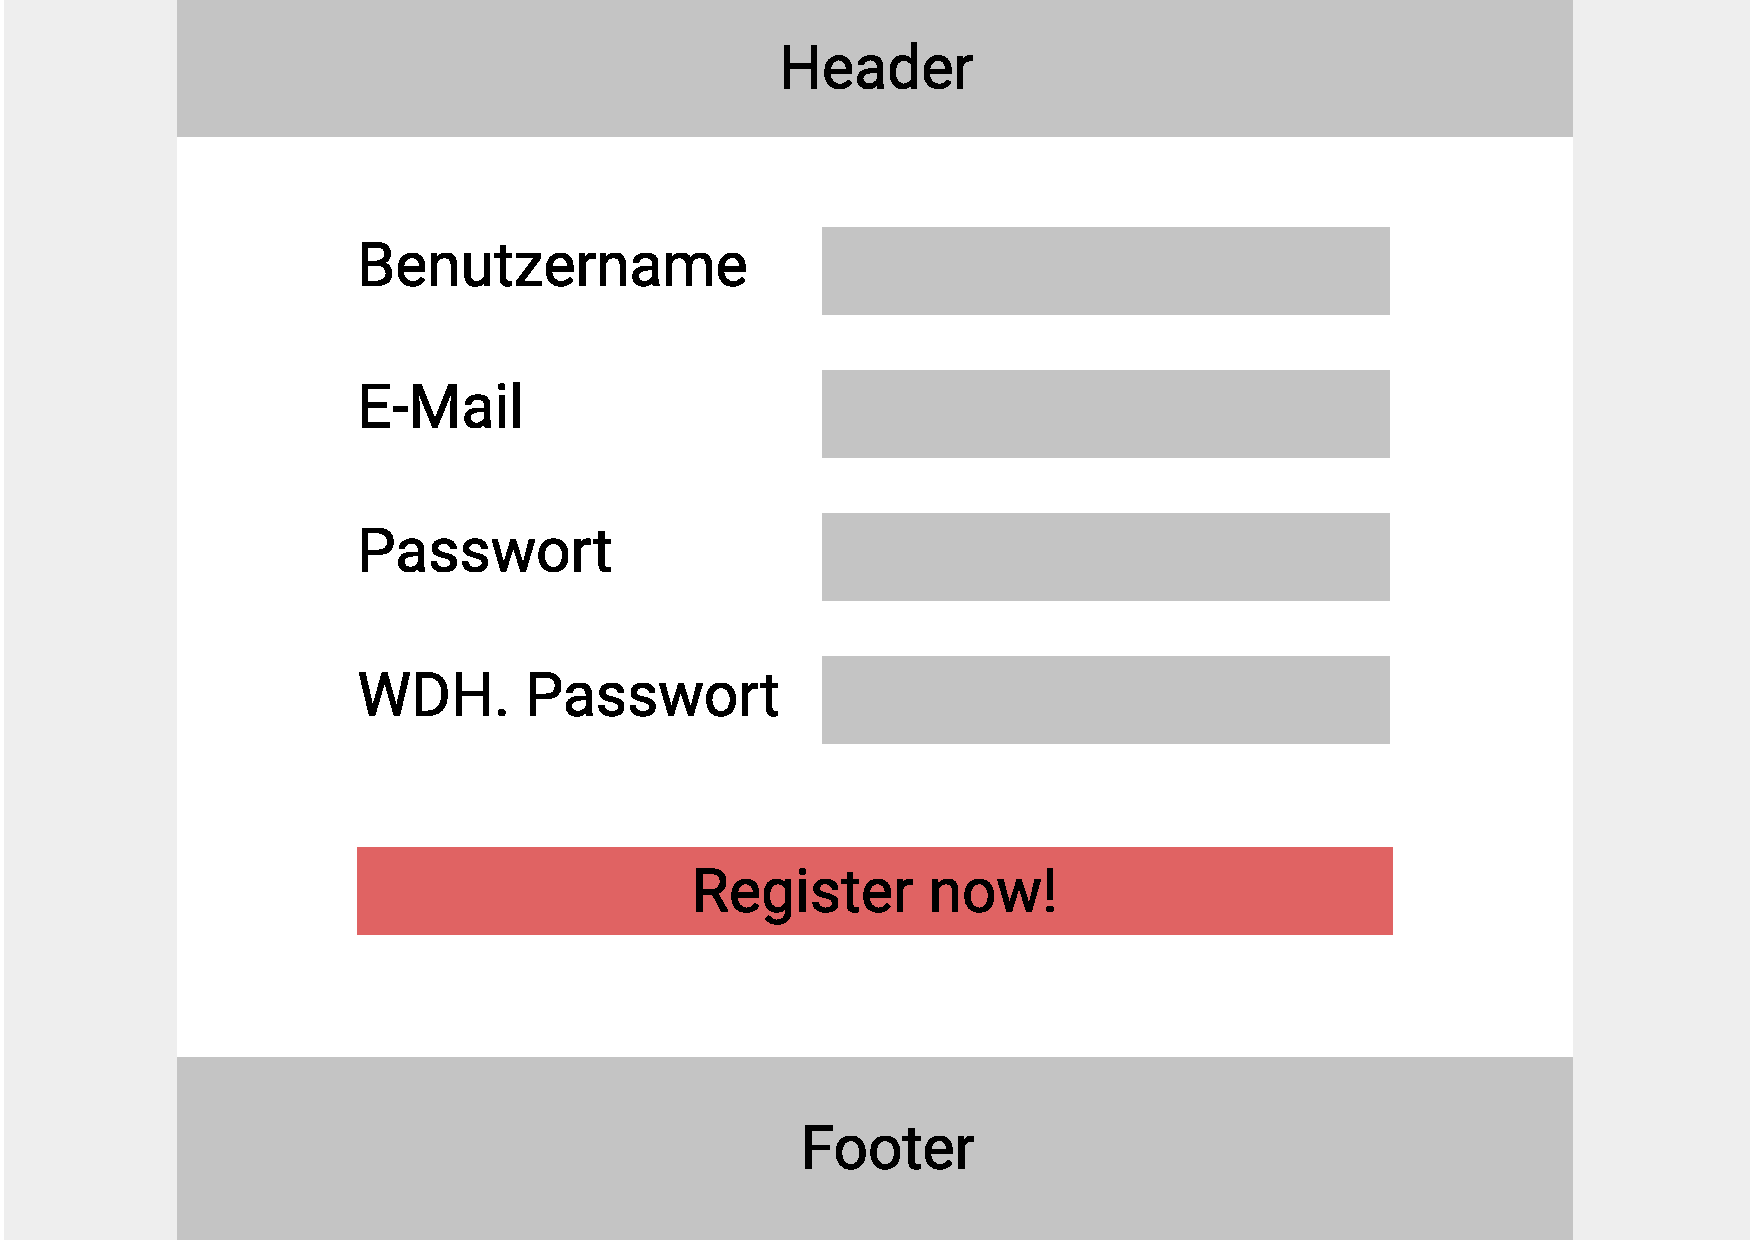
\includegraphics[width=0.7\textwidth]{img/konzeption/client/register}
	\captionsetup{justification=centering, format=plain}
	\caption[Mock-Up der Startseite]{Mock-Up der Registierungsseite \\\figma}
	\label{fig:MockRegister}
\end{figure}